\chapter{Paper I:\@
  Mechanism of \ce{Pd(II)}-mediated\linebreak uncaging reactions % chktex 36
  of propargylic substrates
 }%
\label{ch:paper1}

% TODO: HEY MAYBE REPRODUCE ABSTRACTS\@?

\citetext{Coelho2019}

In order to develop better \ce{C-O} bond cleavage promoters,
recently, bioorthogonal approaches have been devised to promote \ce{C-O} bond
cleavage by trainsition metals for uncaging protected molecules, normally with
hydroxyl and amino functional groups.
Palladium (II) has been extensively used for such biocompatible processes.
Uncaging of propargyl groups has remained challenging.
This reaction has been added to the bioorthogonal arsenal of chemical biology and
medicional chemistry for activating bio and prodrug molecules recently.

It is normally assumed that the process goes through \emph{in situ} formation
of catalytic \ce{Pd(0)}, promoted by a base through intramolecular ligand exchange
reduction or nucleophilic attack by the solvent and then suffering reductive
elimination. This \ce{Pd(0)} could then undergo oxidative addition with the
propargyl group, producing an allenylpalladium intermediate, which is then
hydrolyzed, regenerating the \ce{Pd(0)} and producing acetol as the side product.
A less common hypothetical alternative is the \ce{Pd(II)}-mediated hydration
mechanism to form an intermediate that then decomposes by hydrolisys
(Wacker-like oxidation WHAT IS THIS).

In this work, we attempted to unveil through which mechanism does
the Palladium(II)-mediated chemical uncaging reaction of
progargyl-protected hydroxyl groups takes place.
% TODO: WHICH SUBSTRATES WE USED, RELATE TO COMPUTATION\@?
The reactions were monitored in the lab by UV-vis spectroscopy and a deviation
from first-order kinetics was observed.
A distinct biexponential shape was found, consistent with biphasic kinetics,
which produce the same product (DNP) at different reaction rates.
The fastest reaction has a half-life or 1 hour, and was found to be around 15 times faster than the other, and
650 times faster than the uncatalyzed one.

It was observed that the fast phase was responsible for only two turnovers,
which indicates that, although faster, it shuts down after two turnovers.
Further experiments evidenced that the catalyst may not be stable and is changing through the
course of the reaction, changing its activity.
Furthermore, neither DNP or acetol seem to inhibit the reaction.

With the XAS results, we proceeded to perform computational studies.
We employed the \ce{[PdCl4]2-} complex as the catalyst species, and chose a
model substrate methylpropargyl ether to simplify calculations.
We employed an implicit solvation model in water, and used two explicit extra
water molecules to consider the effect of hydrogen bonding, one interacting
with the enol part and the other with the leaving group.
We used PBE0 to obtain geometries and frequencies, and adjusted the electronic
energy with DLPNO-CCSD(T) and HF-gCP to correct for basis set artifacts.

We found out that both Markovnikov and anti-Markovnikov regiochemical
hydrations of the Pd-propargyl complex to form enols are competitive and within
the method's error (< 1~\kcalmol).
% TODO: CONTINUE FROM THE PARAGRAPH BEFORE FIGURE 4.

Our evidence suggested that the reaction proceeds through biphasic kinetics
with different rates, where the most favorable path involves a \ce{Pd(II)}
anti-Markovnikov hydration of the propargyl group, followed by C-O bond breaking
by $\beta$-O elimination.
The process lasts two turnovers as the product inhibits further
reactivity.

An application to metallocatalysis~\cite{Coelho2019}.
A computational-experimental collaboration.

% TODO:
% HOW IS THE RESEARCH DESIGNED?\@
% WHY IT IS DESIGNED THIS WAY?\@
% WHAT DOES THE LITERATURE SAY ABOUT THIS?\@
% IS THE LITERATURE WELL STABLISHED?\@
% IS IT DIVIDED?\@
% HOW DOES THE RESEARCH FIT THE BIGGER PICTURE?\@
% HOW DOES THE RESEARCH CONTRIBUTE SOMETHING ORIGINAL?\@
% HOW DOES THE METHODOLOGY OF PREVIOUS STUDIES HELP YOU DEVELOP YOUR OWN?\@
% WHY IS THIS WORTH INVESTIGATING?\@
% HOW IMPORTANT IS THIS?\@
% HOW IS THIS ORIGINAL?\@
% WHAT WERE MY RESEARCH AIMS?\@
% WHAT IS THE SCOPE OF MY STUDY?\@
% WHAT I COVERED AND DIDN'T COVER?\@
% WHICH METHODS WERE USED?\@

% TODO:
% \section{Background and motivation}
% PRESENTATION OF THE WORK.\@
% DESCRIPTION OF THE WORK.\@
% OBJECTIVES OF THE WORK.\@
% INTERPRETATION AND MEANING OF THE WORK.\@
% MAIN FINDINGS.\@
% RESULTS IN RELATION TO THE RESEARCH QUESTIONS.\@

\section{Paper}

The publication can be read in full next.

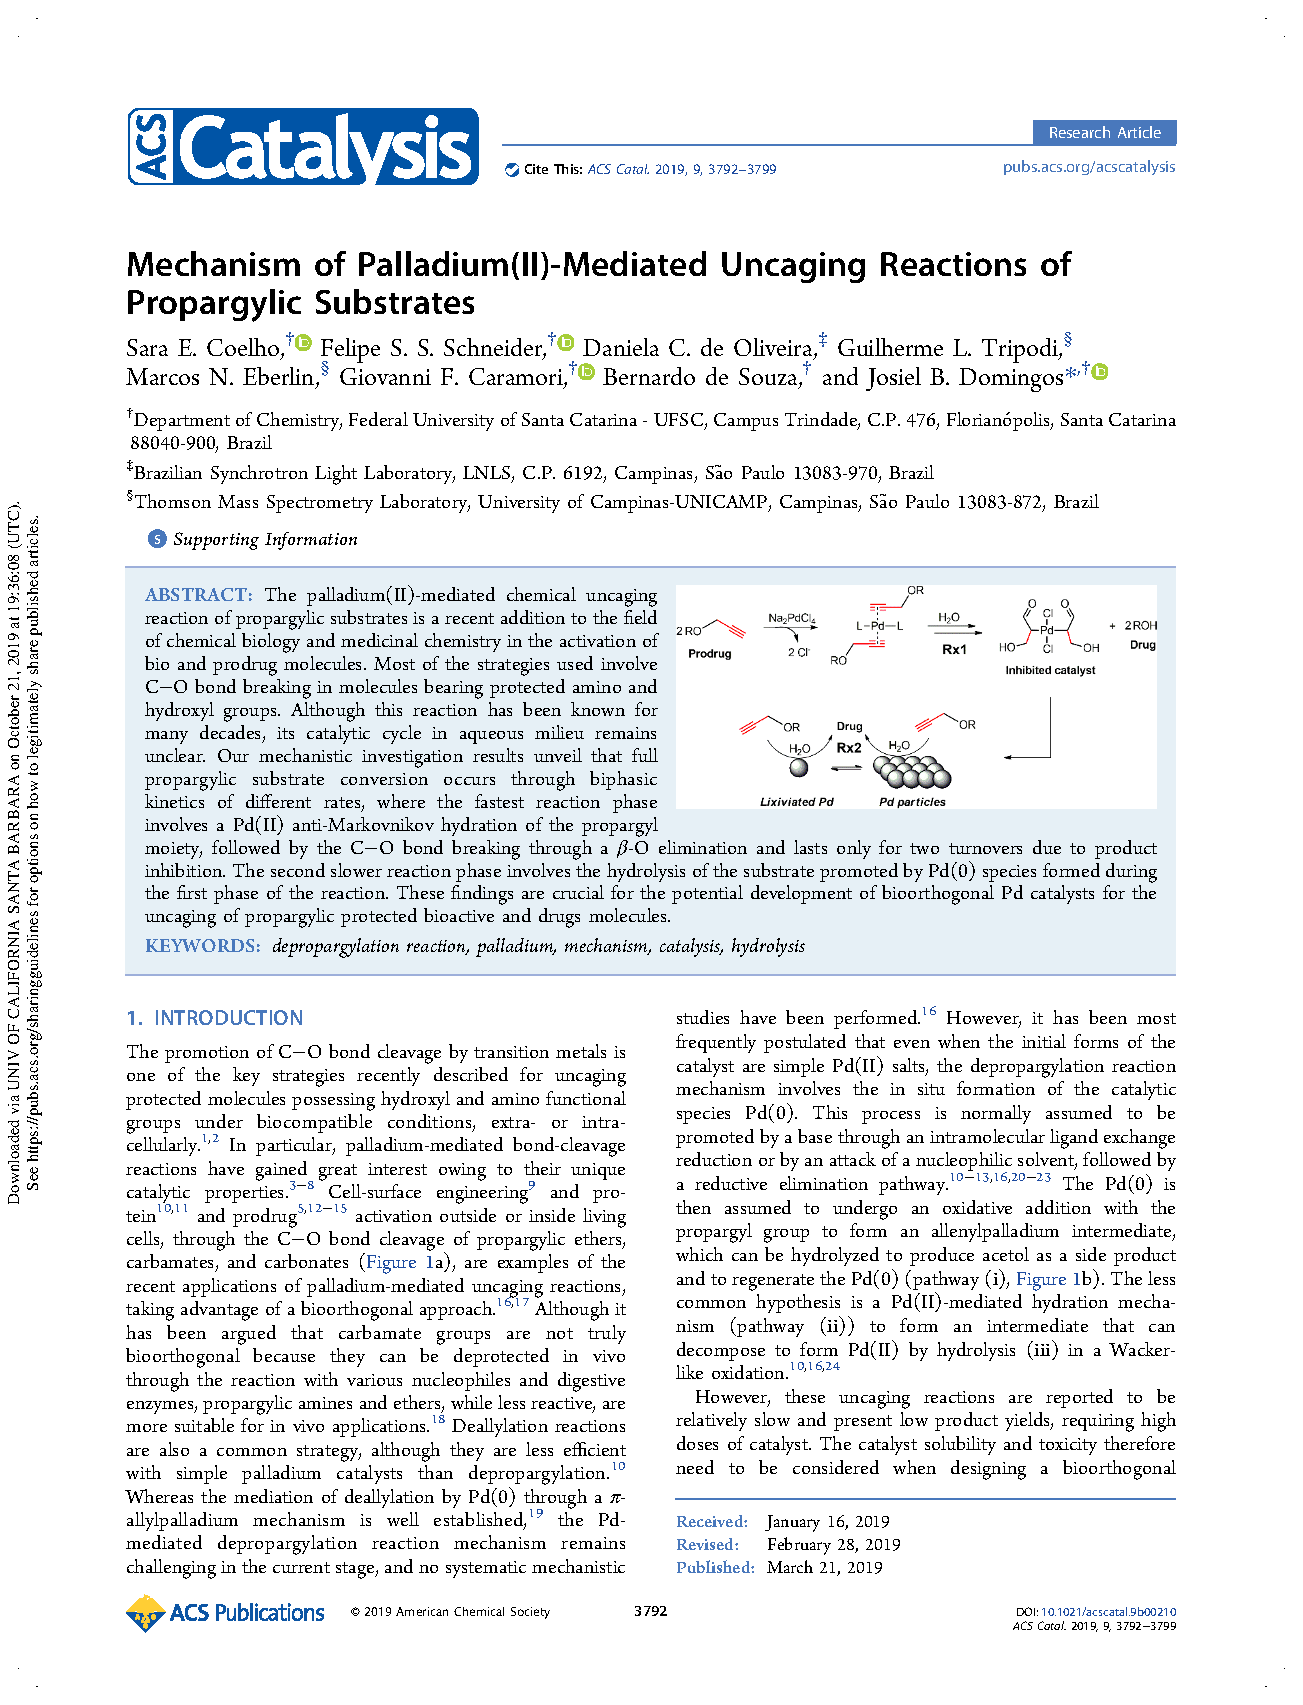
\includepdf[pages=-]{pubs/coelho2019-paper1.pdf}
